\documentclass[11pt]{scrartcl}
\usepackage[T1]{fontenc}
\usepackage[a4paper, left=3cm, right=2cm, top=2cm, bottom=2cm]{geometry}
\usepackage[activate]{pdfcprot}
\usepackage[ngerman]{babel}
\usepackage[parfill]{parskip}
\usepackage[utf8]{inputenc}
\usepackage{kurier}
\usepackage{amsmath}
\usepackage{amssymb}
\usepackage{xcolor}
\usepackage{epstopdf}
\usepackage{txfonts}
\usepackage{fancyhdr}
\usepackage{graphicx}
\usepackage{prettyref}
\usepackage{hyperref}
\usepackage{eurosym}
\usepackage{setspace}
\usepackage{units}
\usepackage{eso-pic,graphicx}
\usepackage{icomma}

\definecolor{darkblue}{rgb}{0,0,.5}
\hypersetup{pdftex=true, colorlinks=true, breaklinks=false, linkcolor=black, menucolor=black, pagecolor=black, urlcolor=darkblue}



\setlength{\columnsep}{2cm}


\newcommand{\arcsinh}{\mathrm{arcsinh}}
\newcommand{\asinh}{\mathrm{arcsinh}}
\newcommand{\ergebnis}{\textcolor{red}{\mathrm{Ergebnis}}}
\newcommand{\fehlt}{\textcolor{red}{Hier fehlen noch Inhalte.}}
\newcommand{\betanotice}{\textcolor{red}{Diese Aufgaben sind noch nicht in der Übung kontrolliert worden. Es sind lediglich meine Überlegungen und Lösungsansätze zu den Aufgaben. Es können Fehler enthalten sein!!! Das Dokument wird fortwährend aktualisiert und erst wenn das \textcolor{black}{beta} aus dem Dateinamen verschwindet ist es endgültig.}}
\newcommand{\half}{\frac{1}{2}}
\renewcommand{\d}{\, \mathrm d}
\newcommand{\punkte}{\textcolor{white}{xxxxx}}
\newcommand{\p}{\, \partial}
\newcommand{\dd}[1]{\item[#1] \hfill \\}

\renewcommand{\familydefault}{\sfdefault}
\renewcommand\thesection{}
\renewcommand\thesubsection{}
\renewcommand\thesubsubsection{}


\newcommand{\themodul}{Messtechnik}
\newcommand{\thetutor}{Prof. Helsper}
\newcommand{\theuebung}{Übung}

\pagestyle{fancy}
\fancyhead[L]{\footnotesize{C. Hansen}}
\chead{\thepage}
\rhead{}
\lfoot{}
\cfoot{}
\rfoot{}

\title{\themodul{}, \theuebung{}, \thetutor}


\author{Christoph Hansen \\ {\small \href{mailto:chris@university-material.de}{chris@university-material.de}} }

\date{}


\begin{document}

\maketitle

Dieser Text ist unter dieser \href{http://creativecommons.org/licenses/by-nc-sa/4.0/}{Creative Commons} Lizenz veröffentlicht.

\textcolor{red}{Ich erhebe keinen Anspruch auf Vollständigkeit oder Richtigkeit. Falls ihr Fehler findet oder etwas fehlt, dann meldet euch bitte über den Emailkontakt.}

\tableofcontents


\newpage

\section{Aufgabe 2.1}

\subsection*{a)}

\begin{align*}
	&\text{linearer Mittelwert:} \qquad \bar{u} = \frac{1}{T} \int u \d t = \unit[0]{V} \\
	&\text{Gleichricht Mittelwert:} \qquad \bar{|u|} = \frac{1}{T} \int |u| \d t = \unit[1]{V} \\
	&\text{effektiver Mittelwert:} \qquad u_{eff} = U = \sqrt{\frac{1}{T} \cdot \int u^2 \d t} = \left(\frac{1}{T} \cdot \left( 1^2 \cdot V^2 \cdot \frac{T}{2} + \left(- \unit[1]{V} \right)^2 \cdot \frac{T}{2} \right) \right)^{0,5} = \unit[1]{V} \\
	\hfill \\
	&\text{Formfaktor:} \qquad F = \frac{U}{|u|} = \frac{\unit{1}[V]}{\unit{1}[V]} = \unit{1}[V]
\end{align*}

\subsection*{b)}

\begin{align*}
	&\text{linearer Mittelwert:} \qquad \bar{u} = \frac{1}{T} \int u \d t = \frac{1}{T} \left(2 \cdot \frac{T}{T} - 1 \cdot \frac{T}{T} \right) = \unit[0,5]{V} \\
	&\text{Gleichricht Mittelwert:} \qquad \bar{|u|} = \frac{1,5}{T} \int |u| \d t = = \frac{1}{T} \left(2 \cdot \frac{T}{T} + 1 \cdot \frac{T}{T} \right) \unit[1]{V} \\
	&\text{effektiver Mittelwert:} \qquad u_{eff} = U = \sqrt{\frac{1}{T} \cdot \int u^2 \d t} = \left(\frac{1}{T} \left(2^2 \cdot \frac{T}{T} + 1^2 \cdot \frac{T}{T} \right) \right)^{0,5} = \unit[1,58]{V} \\
	\hfill \\
	&\text{Formfaktor:} \qquad F = \frac{U}{|u|} = \frac{\unit{1,58}[V]}{\unit{1,5}[V]} = \unit{1,05333}[V]
\end{align*}


\subsection*{c)}

Wir betrachten den Sinus hier als Sinus von x statt von t, da wir dann nicht substituieren müssen.

\begin{align*}
	&\text{linearer Mittelwert:} \qquad \bar{u} = \frac{1}{2 \pi} \int_0^\pi \overset{\wedge}{u} \sin(x) \d x = \overset{\wedge}{u} \cdot \frac{1}{2 \pi} \left[ - \cos(x) \right]_0^\pi = \unit[3,18]{V} \\
	&\text{Gleichricht Mittelwert: Das Signal ist schon gleichgerichtet, deshalb gilt $\bar{u} = |\bar{u}|$}  \\
	&\text{effektiver Mittelwert:} \qquad u_{eff} = U = \sqrt{ \frac{1}{2 \pi} \int_0^\pi \overset{\wedge}{u}^2\sin(x)^2 \d x} = \overset{\wedge}{u} \sqrt{\left[ \frac{1}{2 \pi} \cdot \frac{x - cos(x) \cdot \sin(x)}{2}\right]_0^\pi} = \unit[5]{V} \\
	\hfill \\
	&\text{Formfaktor:} \qquad F = \frac{U}{|u|} = \frac{\unit{5}[V]}{\unit{3,18}[V]} = \unit{1,57}[V]
\end{align*}


\newpage

\subsection*{d)}

Wir müssen in diesem Fall nur bis $\frac{\pi}{2}$ betrachten, weil es sich ab dann schon wiederholt:

\begin{align*}
	&\text{linearer Mittelwert:} \qquad \bar{u} = \frac{2}{\pi} \int_0^\pi \overset{\wedge}{u} \sin(x) \d x = \overset{\wedge}{u} \cdot \frac{2}{\pi} \left[ - \cos(x) \right]_0^\pi = \unit[6,37]{V} \\
	&\text{Gleichricht Mittelwert: Das Signal ist schon gleichgerichtet, deshalb gilt $\bar{u} = |\bar{u}|$}  \\
	&\text{effektiver Mittelwert:} \qquad u_{eff} = U = \sqrt{ \frac{2}{\pi} \int_0^\pi \overset{\wedge}{u}^2\sin(x)^2 \d x} = \overset{\wedge}{u} \sqrt{\left[ \frac{2}{\pi} \cdot \frac{x - cos(x) \cdot \sin(x)}{2}\right]_0^\pi} = \unit[7,07]{V} \\
	\hfill \\
	&\text{Formfaktor:} \qquad F = \frac{U}{|u|} = \frac{\unit{7,07}[V]}{\unit{6,37}[V]} = \unit{1,11}[V]
\end{align*}


\section{Aufgabe 3.1}


\subsection*{a)}

Der Strom durch den Shuntwiderstand $R_S$ heißt $I_S$:

\begin{align*}
R_S &= 90 + 9 + 0,9 + 0,1 = \unit[100]{\Omega} \\
\frac{I_{max}}{I_S} &= \frac{100}{400} \\
\Leftrightarrow I_{max} &= \frac{1}{4} \cdot I_S 
\intertext{Wir wissen das gilt:}
I_{ges} = I_{max} + I_S &= \unit[1]{mA} \Leftrightarrow I_S = \unit[0,8]{mA} \Rightarrow I_{max} = \unit[0,2]{mA}
\end{align*}



\subsection*{b)}

\begin{align*}
\frac{I_{max}}{I_S} &= \frac{0,1}{400 + 99,9} \approx \frac{0,1}{500} \\
\Leftrightarrow I_{max} &= \frac{0,1}{500} \cdot I_S = \frac{I_{ges}}{5000} = \unit[0,2]{mA}
\end{align*}


\newpage

\subsection*{c)}

\begin{figure}[h]
	\centering
	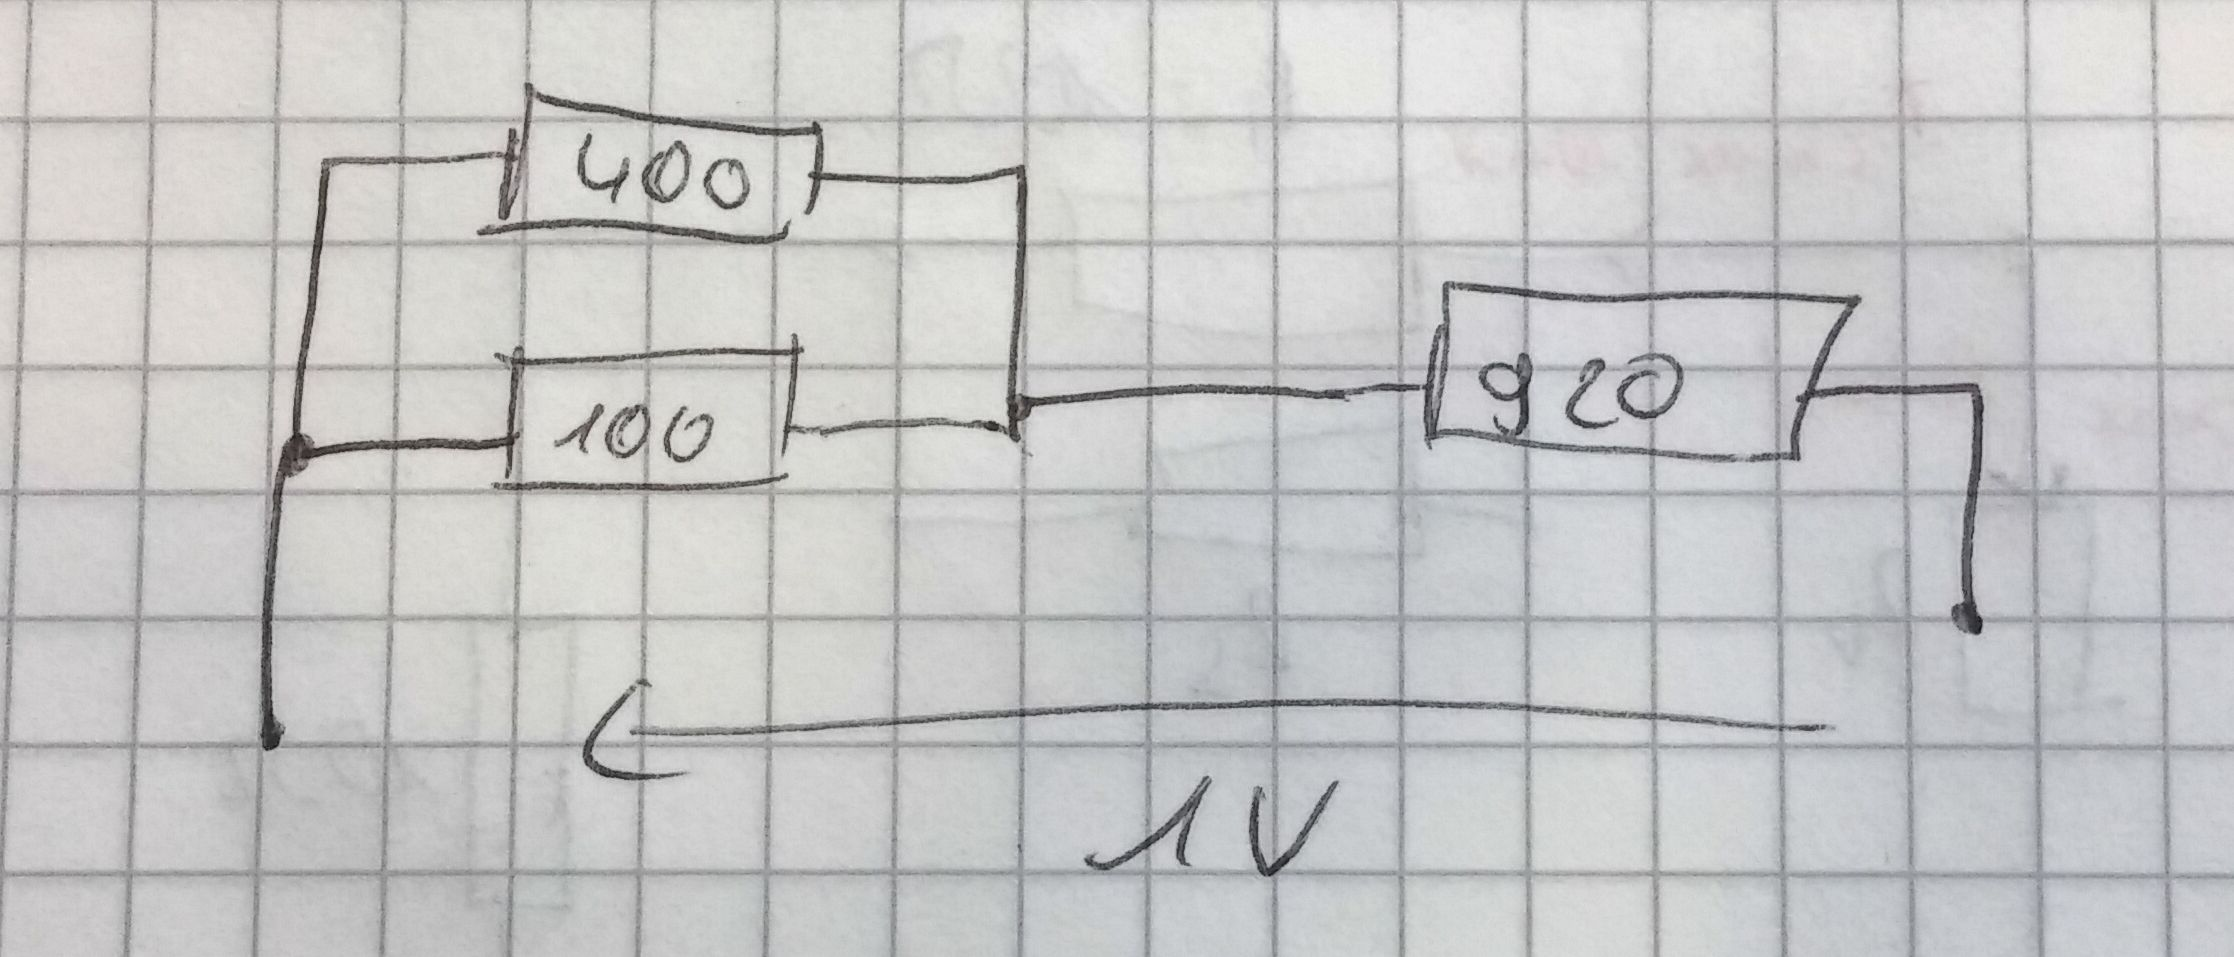
\includegraphics[scale=0.2]{A3_1_1.jpg}
\end{figure}



\begin{align*}
R_{ges} &= 920 + \frac{400 \cdot 100}{400 + 100} = \unit[1000]{\Omega}
\end{align*}


Von dem $\unit[920]{\Omega}$ fließen also \unit[1]{mA} nach links splittet sich dann wie im Aufgabenteil zuvor auf und wir erhalten dann wieder ein $I_{max} = \unit[0,2]{mA}$.

Bei einem $R_{ges} = \unit[100]{k \Omega}$ und $\unit[100]{V}$ haben wir genau die selbe Situation nur andere Werte.


\subsection*{d)}

Die Innenwiderstände sind wie folgt:

\begin{tabular}{|l|l|}
	\hline $\unit[100]{V}$ Messbereich & $\unit[100]{k\Omega}$  \\ 
	\hline $\unit[1]{V}$ Messbereich & $\unit[1]{k\Omega}$ \\ 
	\hline $\unit[1]{mA}$ Messbereich & $\unit[80]{\Omega}$ \\ 
	\hline $\unit[1]{A}$ Messbereich & $\unit[0,1]{\Omega}$ \\ 
	\hline 
\end{tabular} 

\section{Aufgabe 3.2}

Diese Aufgabe wurde nicht gemacht weil sie veraltet ist.

\newpage


\section{Aufgabe 3.3}

\begin{figure}[h]
	\centering
	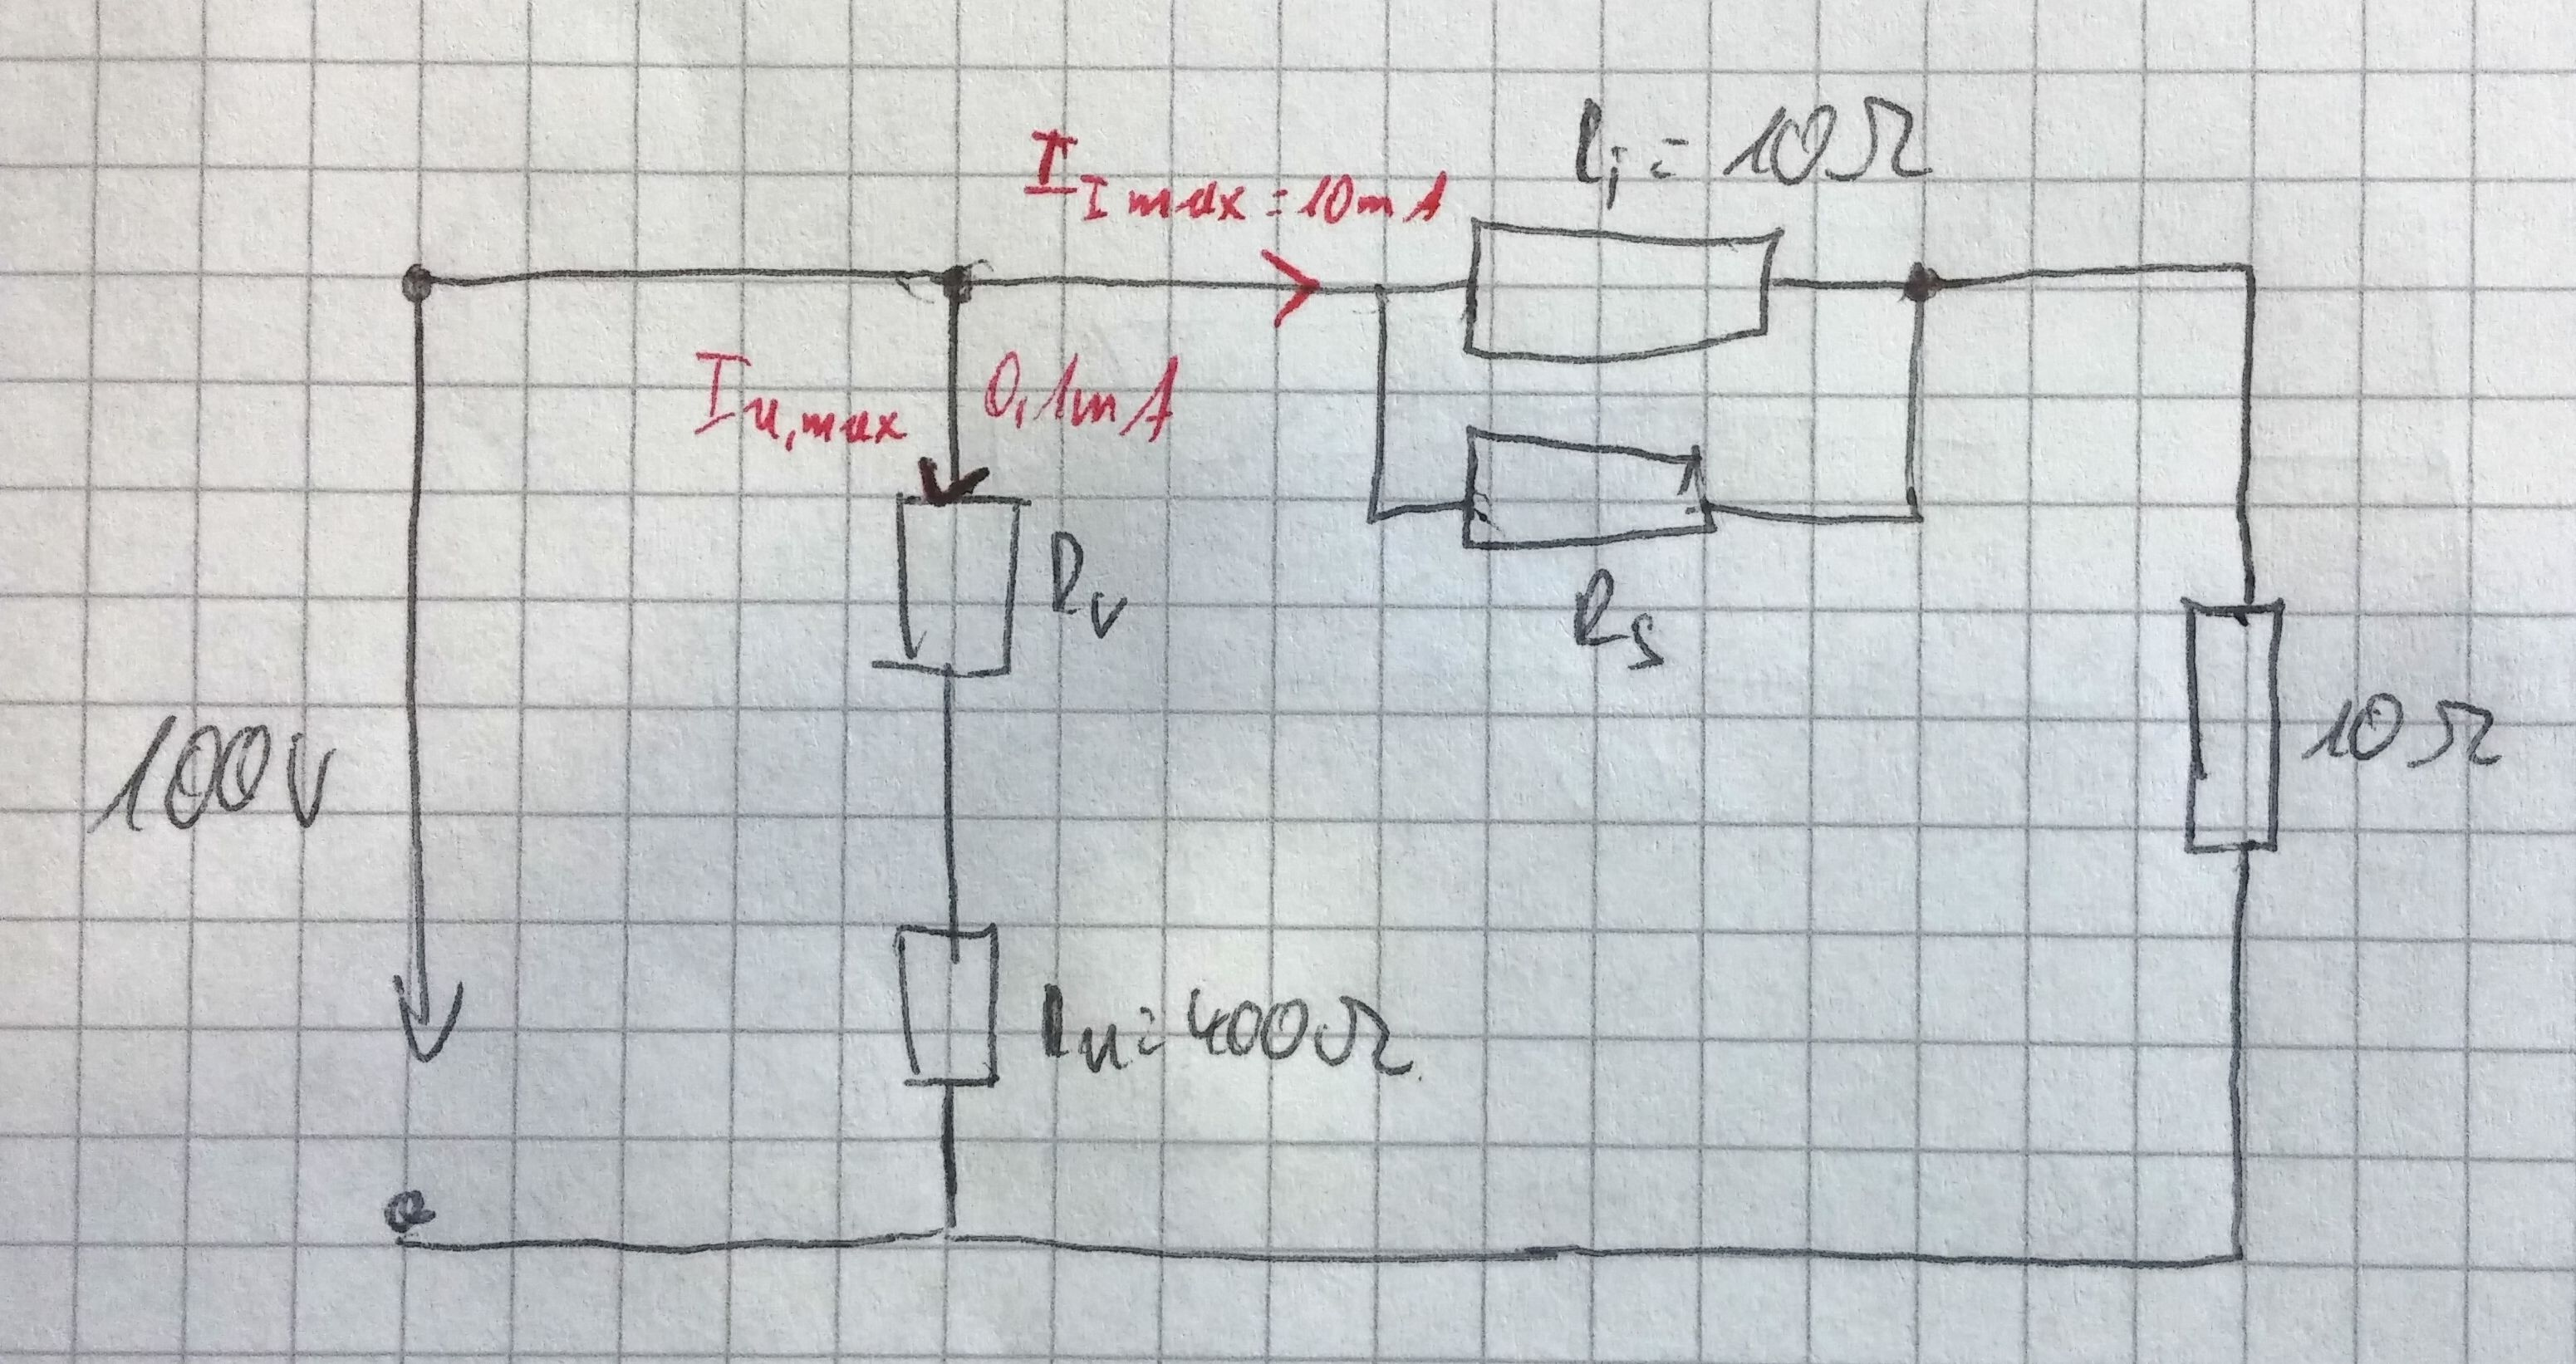
\includegraphics[scale=0.15]{A3_3_1.jpg}
\end{figure}




\begin{align*}
U &= \left( R_V + R_U \right) \cdot I_{U,max} \\
\Leftrightarrow R_V &= \frac{U - R_U \cdot I_{u,max}}{I_{u,max}} = \frac{U}{I_{u,max}} \cdot R_U = \frac{100}{0,1} \cdot 400 = \unit[1]{M \Omega}
\intertext{Nun bestimmen wir noch den Shuntwiderstand:}
\frac{I_S}{I_{I,max}} &= \frac{R_I}{R_S} \Leftrightarrow I_S = \frac{R_I}{R_S} \cdot I_{I,max} \\
I &= I_S + I_{I,max} = I_{I,max} \cdot \left( \frac{R_I}{R_S} + 1 \right) \\
R_S = R_I \cdot \frac{I_{I,max}}{I - I_{I,max}} &= \frac{\unit[10]{mA}}{\unit[10]{A} - \unit[10]{mA}} \cdot \unit[10]{\Omega} = \unit[0,01]{\Omega}
\end{align*}



\section{Aufgabe 4.1}


\subsection*{a)}

Wir berechnen zunächst den Widerstand $R_A$ bei der Strommessung:

\begin{align*}
R_A &= \frac{\unit[200]{mV}}{\unit[20]{A}} = \unit[0,01]{\Omega}
\intertext{Zur Abschätzung des Innenwiderstands $R_Q$ tun wir so als wäre die Messung korrekt:}
R_Q = \frac{U_V}{I_A} &= \frac{1,2}{13,33} = \unit[0,09]{\Omega}
\intertext{Der Widerstand ist also um etliche Größenordnungen kleiner als $R_V$ und daher können wir die Spannungsmessung als genau annehmen $U_0 = U_V$. Nun bestimmen wir den Widerstand bei der Strommessung:}
I_A &= \frac{U_0}{R_Q + R_A} \\
\Leftrightarrow U_0 &= I_A \cdot R_Q + I_A \cdot R_A \\
\Leftrightarrow R_Q = \frac{U_0 - I_A \cdot R_A}{I_A} &= \frac{1,2 - 13,33 \cdot 0,01}{13,33} = \unit[0,08]{\Omega}
\end{align*}

\subsection*{b)}

Es macht keinen Sinn bei der Spannung einen Fehler zu berechnen, weil der Fehler auf Grund des großen Widerstandes weit kleiner ist als das Messgerät anzeigen kann.

Für den Strom können wir den Fehler so berechnen:

\begin{align*}
I_K &= \frac{U_0}{R_Q} = \frac{1,2}{0,08} = \unit[15]{\Omega} \\
e &= I_A - I_K = \unit[- 1,67]{A} \\
e^* &= \frac{e}{I_K} = \frac{-1.67}{15} = -0,111 = \unit[-11,1]{\%}
\end{align*}


\section{Aufgabe 4.2}

Der Widerstand $R_h$ ist ein \textbf{einstellbarer} Widerstand, da mit diesem Widerstand kompensiert werden soll. Wir bestimmen zunächst de minimalen und den maximalen Strom:

\begin{align*}
I_{K,max} &= \frac{\unit[5]{V}}{\unit[50]{\Omega}} = \unit[0,1]{A} \\
I_{K,min} &= \frac{\unit[5]{V}}{\unit[200]{\Omega}} = \unit[0,025]{A}
\intertext{Die zugehörigen minimalen und maximalen Widerstände sind dann:}
R_{h,max} &= \frac{\unit[10]{V}}{\unit[0,025]{A}} = \unit[400]{\Omega} \\
R_{h,min} &= \frac{\unit[10]{V}}{\unit[0,1]{A}} = \unit[100]{\Omega}
\intertext{Die Genauigkeit muss sich als an dem kleineren Widerstand orientieren:}
\Delta R_{h,min} &= 100 \cdot 0,001 = \unit[0,1]{\Omega}
\intertext{Jetzt stellt sich die Frage wie sich die Spannung an dem Widerstand $R_S$ ändert, wenn wir den Wert von $R_h$ um eine Einheit aus der Kompensationsstellung verstellen:}
U_M &= (I - I_h) \cdot R_S = I \cdot R_S - \frac{U_h}{R_h} \cdot R_S
\intertext{Dazu müssen wir die obige Formel ableiten:}
\frac{\p U_M}{\p R_h} &= \frac{U_h}{R_h^2} \cdot R_S \\
\Rightarrow \Delta U_M &= \frac{U_h \cdot R_S}{R_h^2} \cdot \Delta R_h = \frac{\unit[10]{V} \cdot \unit[10^3]{\Omega}}{\left( \unit[100]{\Omega} \right)^2} \cdot \unit[0,1]{\Omega} = \unit[0,1]{V}
\end{align*}


\section{Aufgabe 4.3}

Diese Aufgabe ist nicht klausurrelevant und wurde noch nicht in der Übung besprochen.


\section{Aufgabe 4.4}

\begin{figure}[h]
	\centering
	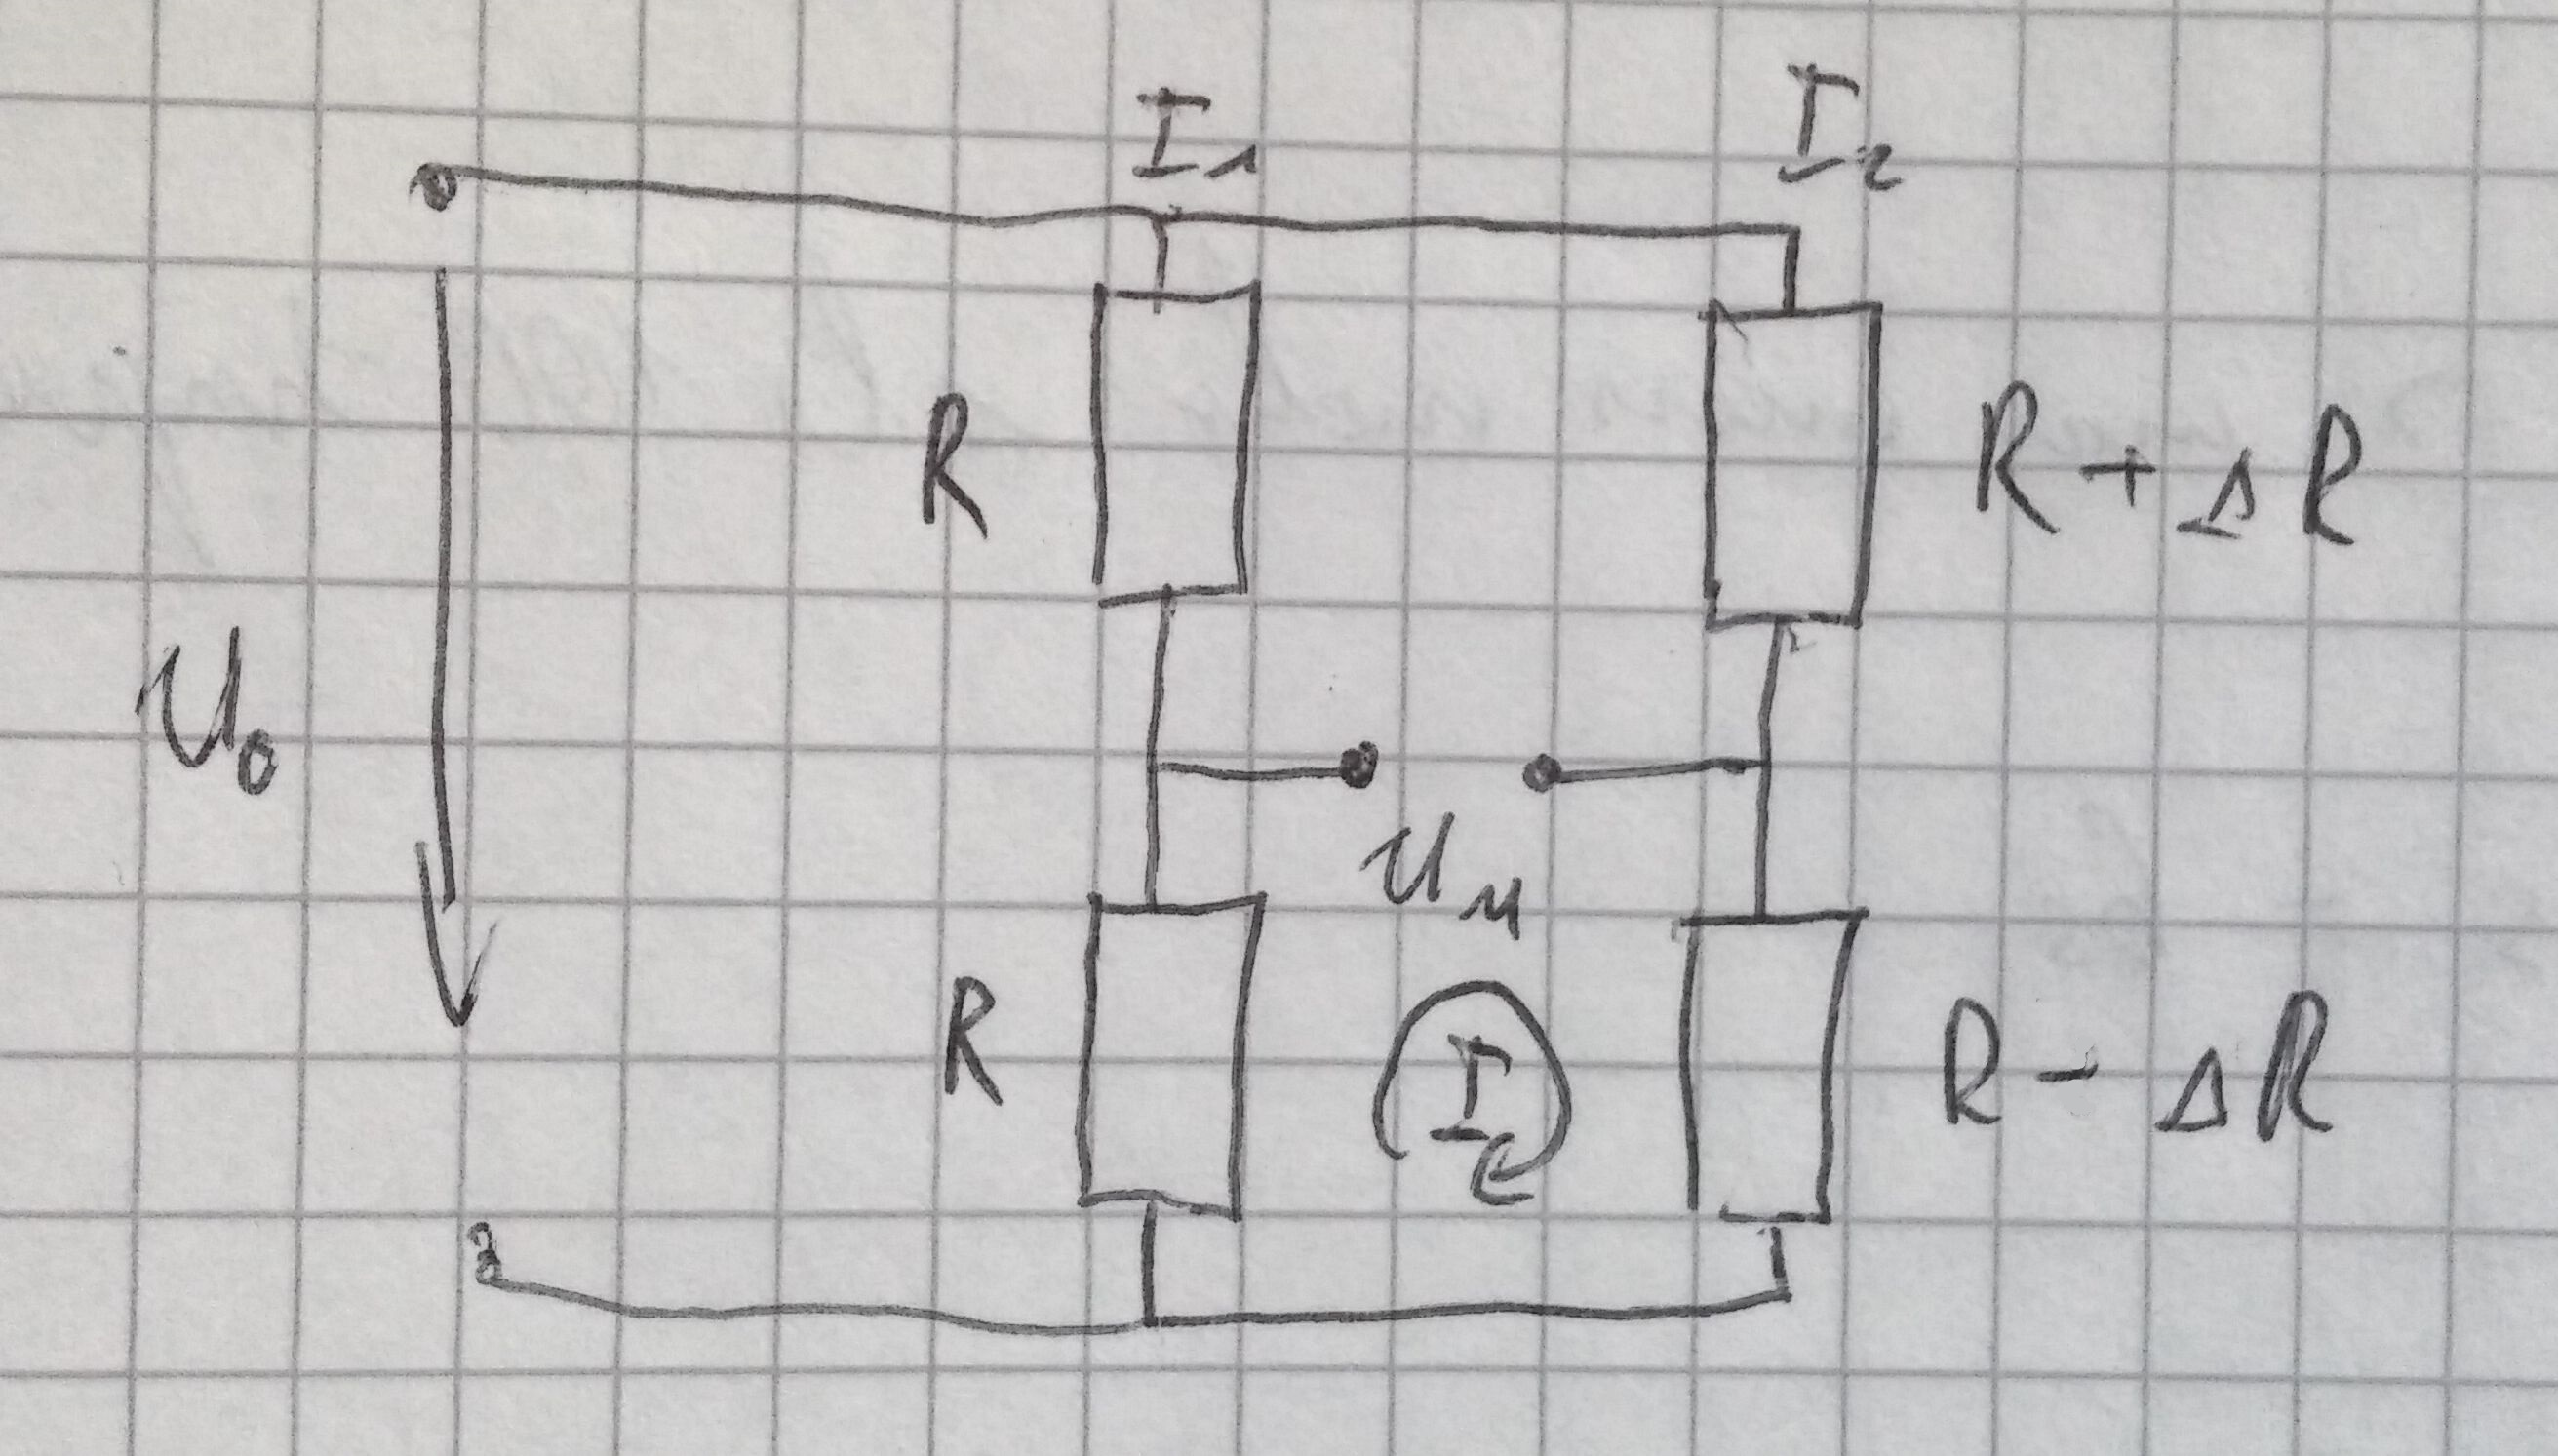
\includegraphics[scale=0.1]{A4_4_1.jpg}
\end{figure}


\subsection*{a)}

Wir wollen die Empfindlichkeit der Messbrücke bestimmen. Die Empfindlichkeit hängt dabei folgendermaßen von der Spannungsänderung und der Dehnung ab:

\begin{align*}
E &= \frac{\Delta U_M}{\Delta \epsilon} = ?
\intertext{Zunächst drücken wir die Spannung $U_0$ mit den zwei möglichen Ästen ab:}
U_0 &= R_1 \cdot I_1 + R \cdot I_1 = 2 R T_1 \\
U_0 &= \left( R + \Delta R \right) \cdot I_2 + \left( R - \Delta R \right) \cdot I_2 = 2 R I_2 
\intertext{Nun könen wir nach dem Strom lösen:}
I = I_1 = I_2 &= \frac{U_0}{2 R} \\
\intertext{Wir betrachten den Maschenumlauf I:}
U_M &= I \cdot \left( R- \Delta R \right) - I \cdot R = 0 \\
\Leftrightarrow U_M &= I \cdot \Delta R = \frac{U_0}{2} \cdot \frac{\Delta R}{R}
\intertext{Das Verhältnis $\frac{\Delta R}{R}$ hängt direkt mit dem k-Faktor und der Dehnung zusammen:}
\frac{\Delta R}{R} &= k \cdot \epsilon \Rightarrow U_M = \frac{U_0}{2} \cdot k \cdot \epsilon 
\intertext{Die Empfindlichkeit ist die Ableitung dieser Gleichung nach der Dehnung:}
E &= \frac{\p U_M}{\p \epsilon} = \frac{U_0}{2} \cdot k = \frac{20}{2} \cdot 2 = \unit[20]{V}
\end{align*}

\subsection*{b)}

\begin{align*}
U_M &= \frac{20}{2} \cdot 2 \cdot 2 \cdot 10^{-4} = \unit[4]{mV}
\end{align*}


\section{Aufgabe 4.5}

Zunächst bestimmen wir die Impulsfrequenz:

\begin{align*}
f_s &= \frac{1000}{60} = \unit[16,7]{1/s}
\intertext{Damit der Fehler unter $\unit[1]{\%}$ liegt müssen wir mehr als 100 Impulse messen:}
T_{ref} &= \frac{100}{16,7} = \unit[5,98]{s}
\end{align*}

In der Praxis kann man sowas nicht verwenden, da die Totzeit viel zu groß ist.








\end{document}